\documentclass[../../main.tex]{subfiles}


\begin{document}

\section{Pedal de Distorsión}

\subsection{Introducción}

Se busca implementar un pedal de distorsión para guitarra eléctrica. La distorsión a implementar ser\'a de tipo clipping, utilizando diodos para efectuar tal distorsión.
Las señales de audio se manejan con niveles de tensión, que representan directamente la onda de entrada, en nuestro caso proveniente de una guitarra eléctrica. Es luego de la conversión de esta onda sonora a una eléctrica que se realizan los cambios de tensión que darán los efectos distorsionantes deseados al sonido.  La señal eléctrica ser\'a nuevamente convertida a audio y ser\'a la salida de cualquier dispositivo reproductor de audio de elección que caiga dentro de las consideraciones que se enumerarán en la subsección \nameref{disenoCirc}.\par %link a diseño del circuito

A modo de delimitar un marco teórico y notacional a partir del cual se presentarán con mayor claridad y precisión los efectos del pedal, se procede a definir el concepto de distorsión a través de la ausencia de la misma: \par

\begin{itemize}
	\item Un sistema con entrada x(t) y salida y(t) no distorsiona cuando y(t) = A x(t+{$\uptau$}), con A y {$\uptau$} dos constantes.  En caso de que esta relación entre entrada y salida no se cumpla, se dice que el sistema en cuestión distorsiona.\par
\end{itemize}

De la definición anterior se desprende que un amplificador operacional ideal cuya entrada $V_d$ = $V^{\text{+}}$ - $V^{\text{-}}$ no supere los valores de saturación característicos y que tenga comportamiento lineal en amplitud y en fase podrá ser clasificado como un amplificador puro y por lo tanto comprenderá un sistema no distorsionante. \par
La distorsión de tipo clipping consiste en el establecimiento de un valor de tensión "techo" o límite, el cual la señal de entrada no podrá sobrepasar en su forma original (sufrirá distorsión). En general, la distorsión será en amplitud, de modo que la salida del sistema y(t) tenderá a valores de tensión cercanos a los del valor techo en aquellos casos en los que la entrada x(t) supere dicho valor. Cabe destacar que en el caso del pedal implementado, el valor techo utilizado será una cota del módulo de la señal de entrada tal que si T es el valor techo,  $|x(t)|\le T$ . Este tipo de clipping se llama clipping simétrico.
De esta forma,  se puede diferenciar entre dos tipos de clipping, a saber:  \par

\begin{enumerate}

\item \underline{\textbf{Hard-Clipping}}: El valor techo del clipping no podrá ser excedido por la señal de salida, y en caso de que la señal de entrada sea superior al valor techo, la señal de salida adoptará el valor constante del techo. Matemáticamente: \par
	%hard clipping expresión matemática.
	 \begin{equation}
    	 \label{eq:aqui-le-mostramos-como-hacerle-la-llave-grande}
  	   y(t) = \left\{
	  	    \begin{array}{ll}
		 					T      & \mathrm{si\ } x(t) \ge T \\
			 				x(t) & \mathrm{si\ } -T \le x \le T \\
			 				-T     & \mathrm{si\ } x(t) \le -T
	     	 \end{array}
	     	\right.
 	\end{equation}
\par
De esta definición se muestra el efecto de clipping sobre una senoidal:

\begin{figure}[H]	%ejemplo hard clipping
	\centering
	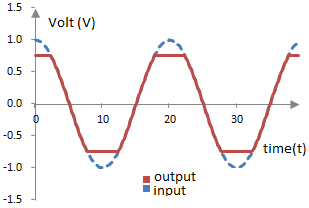
\includegraphics[scale=1]{imagenes/hard_clipping_grafico_tipico.png}
	\caption{Ejemplo de hard-clipping}
	\label{fig:ej5_hard_clipping_grafico_tipico}
\end{figure}

\item \underline{\textbf{Soft-Clipping}}: El valor techo del clipping podrá ser levemente excedido de manera tal que la transición entre el valor que adoptaría la señal de entrada sin distorsión y el que deberá adoptar la señal de salida sea más suave.\par

\begin{figure}[H]	%ejemplo soft clipping
	\centering
	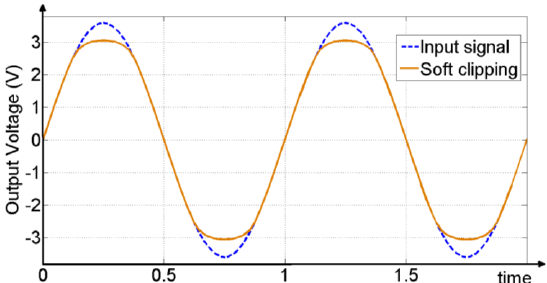
\includegraphics[scale=0.4]{imagenes/soft_clipping_grafico_tipico.png}
	\caption{Ejemplo de soft-clipping}
	\label{fig:ej5_soft_clipping_grafico_tipico}
\end{figure}


\begin{figure}[H]	%soft clipping vs hard clipping
	\centering
	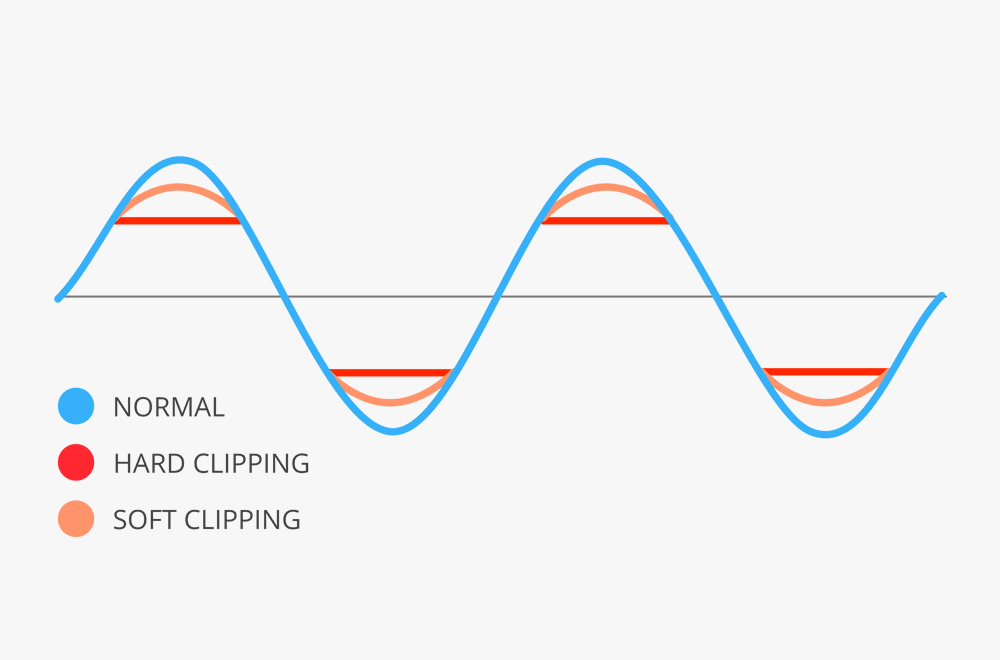
\includegraphics[scale=0.2]{imagenes/hard_clipping_vs_soft_clipping.png}
	\caption{Soft-clipping vs. Hard-clipping}
	\label{fig:ej5_hard_clipping_vs_soft_clipping}
\end{figure}

\end{enumerate}
\subsection{Consideraciones de dise\~no} \label{ssec:ej5_consideraciones_disenio}
Antes de comenzar con el diseño, se definen las asumpciones iniciales sobre las zcuales se comenzará con el diseño del circuito. Estas asumpciones son elegidas de forma tal que se pueda abarcar un gran espectro de las guitarras y aplificadores comerciales.\par
\begin{itemize}
	\item La entrada ser\'a una señal de audio (20Hz a 20KHz) de amplitud menor o igual a 300mV pico a pico (dentro de esta categoria caen la mayor\'ia de los micr\'ofonos de guitarra el\'ectrica). La entrada en principio tendrá offset nulo.
	\item La salida debe ser adecuada para un equipo de audio, por lo que tampoco tendrá tensión de offset continuo.
	\item La fuente de alimentaci\'on debe ser de 9V no partida. De usar un AC ADAPTER, se debe considerar que suele tener un ripple no deseado producto de la conversi\'on no ideal de alterna a continua.
	\item La salida se conectar\'a a un amplificador de guitarra con impedancia de entrada $Z_{in}$ mayor o igual a $200K\Omega$\todo{Zin: hay amplis con Zin mucho mas baja, tipo 44K. Nos falta hacer las cuentas que onda en ese caso, pero creo que nos jode}. Esto es el caso en la mayor\'ia de los amplificadores de guitarra, como por ejemplo la serie Mustang GT de Fender y la serie Cube de Roland, los cuales tienen $Z_{in} = 1M\Omega$, o el Fender Rumble para bajo, con $Z_in = 202K\Omega$ 
	\item La se\~nal de entrada provendr\'a de una guitarra el\'ectrica con impedancia de salida menor a quinchimil millones de ohms.\todo[inline]{Buscar Zout guitarras}	
\end{itemize}


\subsection{Dise\~no del circuito}
\label{disenoCirc}
El circuito con el cual se impondrá la distorsión, con los valores todavía sin definir, es:

\begin{figure}[H]	%esquemático sección alimentación
	\centering
	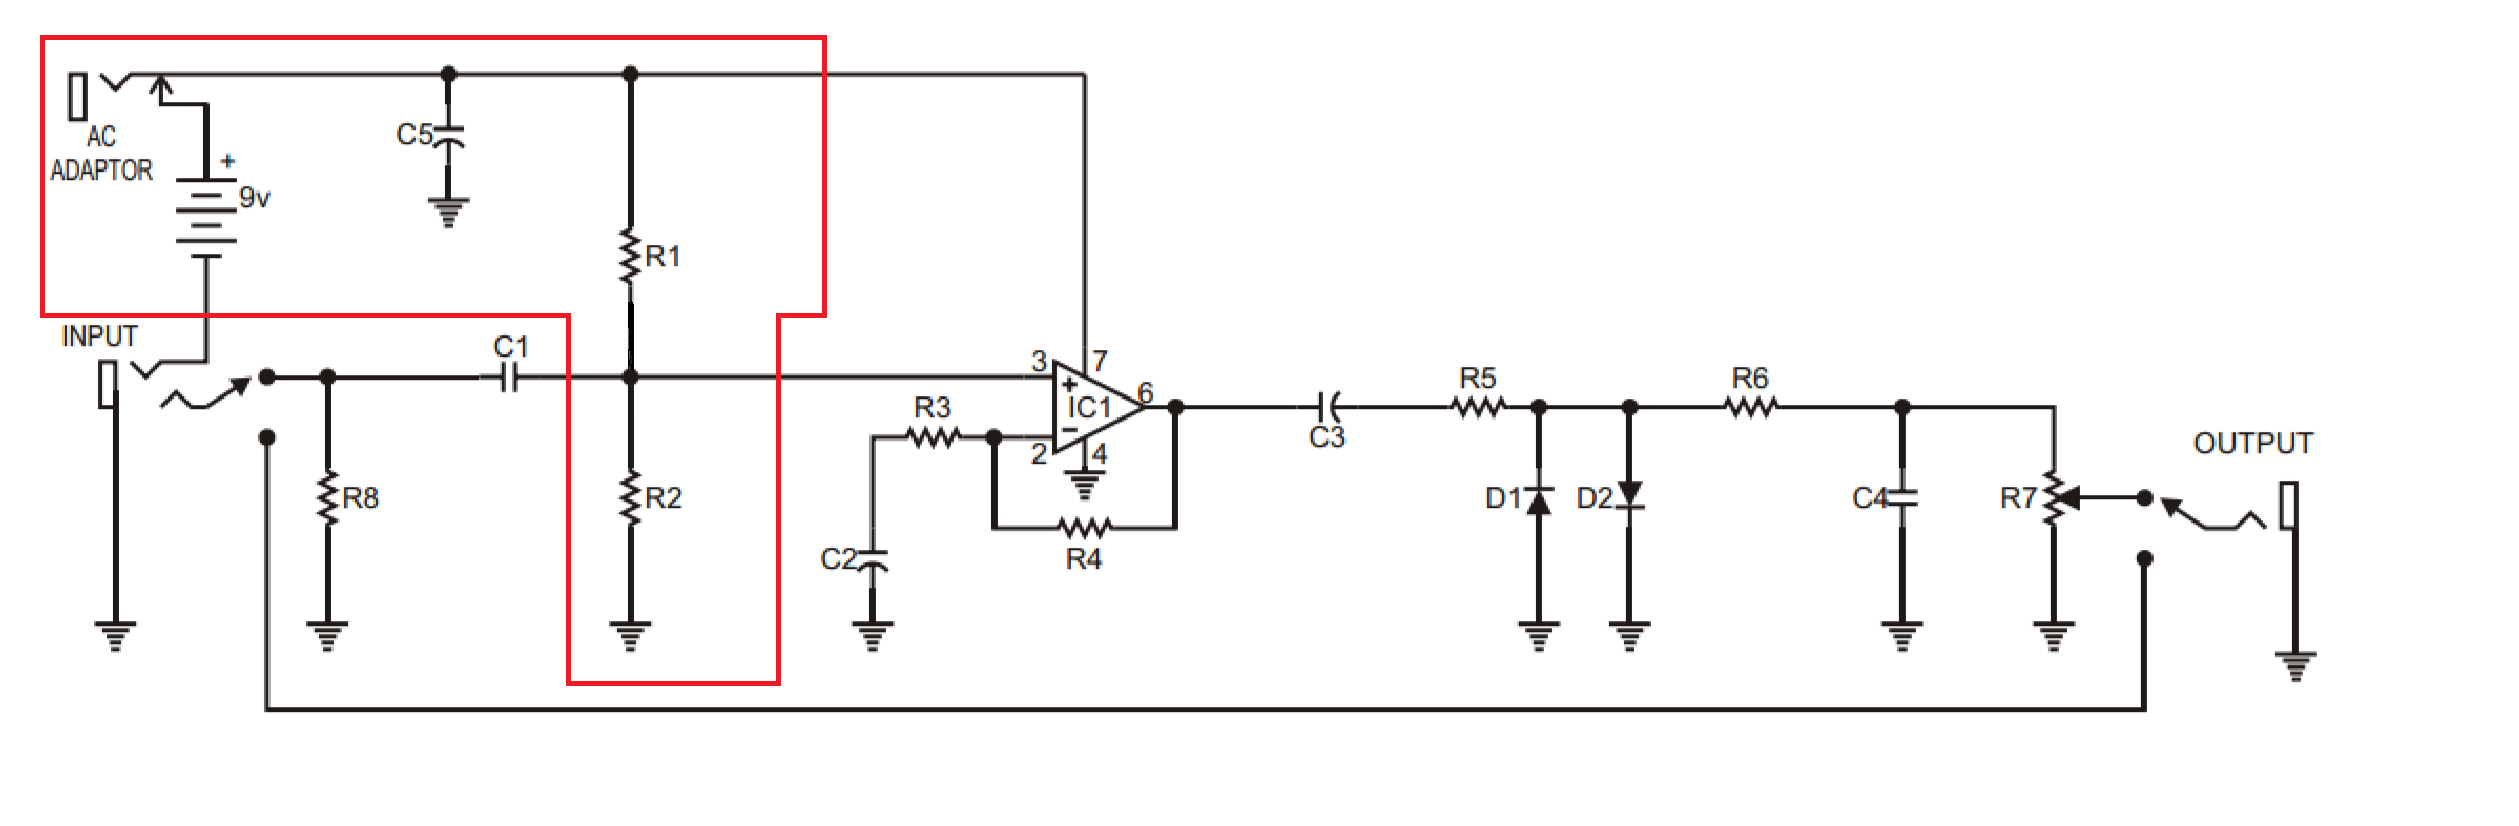
\includegraphics[scale=0.6]{imagenes/Circuito_consigna.png}
	\caption{Circuito de distorsión de clipping a implementar para el pedal de guitarra.}
	\label{fig:ej5_Circuito_consigna}
\end{figure}

Este circuito cuenta con tres secciones notables a saber: 
\begin{enumerate}
\item Alimentación.
\item Amplificación.
\item Clipping.
\end{enumerate}
La numeración de las secciones se corresponde con la imagen anterior. Cada una puede analizarse independientemente tomando los recaudos necesarios.

\subsubsection{Caracter\'isticas del amplificador}
\subsubsection{Secci\'on de alimentaci\'on}

Con el objetivo de minimizar tanto el espacio ocupado por el pedal como la cantidad de baterías requeridas por el usuario para utilizarlo, se busca que el amplificador operacional (opamp) requerido para amplificar la señal de entrada sea alimentado únicamente por una batería en el extremo Vcc+, mientras que el otro extremo de alimentación esté conectado directamente a tierra, de esta manera se "ahorra" una batería, que en este caso en particular será de 9 volts por el tipo de señal con el que se trata. \par 
El problema de este tipo de alimentación es que si la señal de entrada oscila alrededor del 0V, el opamp saturará cuando se rodee estos valores, por lo que la señal será completamente distorsionada de una manera no deseada. Como solución, se plantea montar a la señal de entrada sobre una continua de 4.5 V, por lo que si la señal original cumple con las consideraciones de diseño mencionadas en la sección anterior, el opamp no se saturará si se lograse evitar amplificar la continua sobre la cual se la monta. \par
Es así como para la alimentación se propone el siguiente sub-circuito:

\begin{figure}[H]	%esquemático sección alimentación
	\centering
	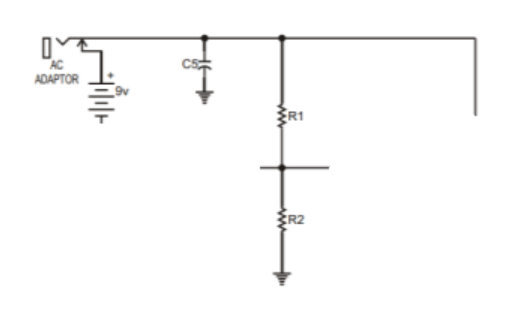
\includegraphics[scale=1]{imagenes/esquematico_alimentacion.png}
	\caption{Esquem\'atico secci\'on de alimentaci\'on}
	\label{fig:ej5_esquematico_alimentacion}
\end{figure}


En el caso en que $R_1$ = $R_2$, las dos resistencias crean un divisor resistivo con el cual se obtienen nodos 9V, 4.5V, y 0V. Esto funciona correctamente siempre que la corriente que circula por ambas resistencias no sea significativamente distinta, ya que en caso contrario la tensión que debería ser de 4.5V va a tomar otro valor. 
\todo{explicar un poquito mejor esto de las corrientes porque no es a prueba de dummies (no aprobó la prueba "Tommy entender")}
La función del capacitor es eliminar cualquier ruido o ripple presente en la tensi\'on de entrada. El ripple es producto del m\'etodo de funcionamiento de los transformadores de alterna a continua (anexo). Una fuente de ruido es ~~~\todo{describir minimamente ac->dc y como genera ripple y poner en el anexo, y poner una fuente de ruido si amerita.}\par
Otra causa de ripple para la fuente de continua se dará en aquellos casos en los que el opamp demande corriente abruptamente, en cuyo caso, dado que la batería no es ideal, no podrá mantener la tensión completamente constante. Este problema se soluciona con el agregado del capacitor $C_5$, que acumulará carga podrá aportar tensión cuando aparezca el riple, manteniendo la tensión continua. Es claro ver que la impedancia del camino a tierra que produce $C_5$ disminuye cuanta más alta sea la frecuencia, por lo que fluctuaciones más grandes en tensión irán directamente a tierrra en vez de influir en el resto del circuito.\par
Dado que los cambios en la demanda de corriente por parte del opamp pueden ser significativamente abruptos, se busca un capacitor que pueda acumular una carga acorde (alta capacitancia, en nuestro caso 1$\mu$F). 

\subsubsection{Secci\'on de clipping}

\begin{figure}[H]	%esquematico seccion clipping
	\centering
	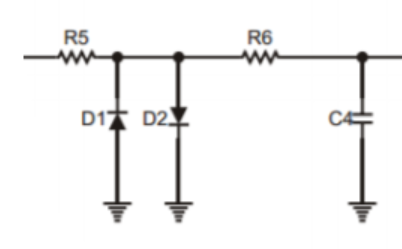
\includegraphics[scale=1]{imagenes/esquematico_clipping.png}
	\caption{Esquem\'atico secci\'on de clipping}
	\label{fig:ej5_esquematico_clipping}
\end{figure}

Esta secci\'on del circuito distorsiona la se\~nal recortando abruptamente cualquier pico que se exceda del rango $\pm$0.6V (si no se excede, no se modifica). Este proceso, explicado en al introducción, se conoce como clipping (ver figura \ref{fig:ej5_diode_clipping}).
El efecto de clipping genera un aumento en los arm\'onicos de alta frecuencia ya que la se\~nal tiende a la forma de una cuadrada en sus picos más altos. Como se mencionó en la introducción, se decidi\'o usar clipping sim\'etrico al elegir acotar el módulo de la señal de entrada por T = 0.6V.

\begin{figure}[H]		%diode clipping (a)simetrico
	\centering
	\begin{subfigure}[b]{0.45\textwidth}
		\centering
		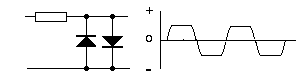
\includegraphics[scale=.8]{imagenes/diode_clipping_symmetrical.png}
		\caption{}
		\label{fig:ej5_diode_clipping_sym}
	\end{subfigure}
	\begin{subfigure}[b]{0.45\textwidth}
		\centering
		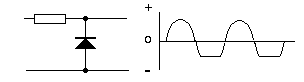
\includegraphics[scale=.8]{imagenes/diode_clipping_asymmetrical.png}
		\caption{ }
		\label{fig:ej5_diode_clipping_asym}
	\end{subfigure}
	\caption{Dos tipos de clipping con diodos: sim\'etrico (\ref{fig:ej5_diode_clipping_sym}) y asim\'etrico (\ref{fig:ej5_diode_clipping_asym})}
	\label{fig:ej5_diode_clipping}
\end{figure}

\subsubsection{Secci\'on de amplificaci\'on}

\begin{figure}[H]	%esquematico seccion amplificacion
	\centering
	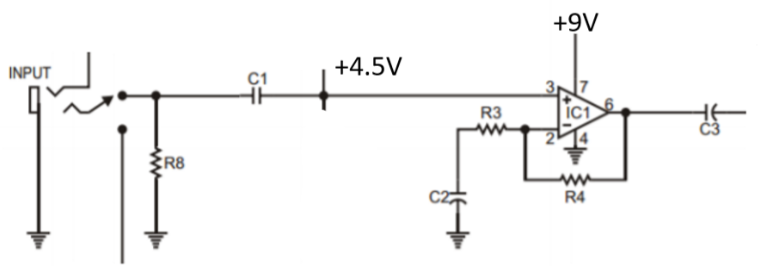
\includegraphics[scale=1]{imagenes/esquematico_amplificacion.png}
	\caption{Esquem\'atico secci\'on de amplificai\'on}
	\label{fig:ej5_esquematico_amplificacion}
\end{figure}

Dado que la alimentaci\'on no es partida, se alimenta el amplificador con Vcc$^-=0$V y Vcc$^+=$9V, lo cual genera la necesidad de montar la se\~nal de audio sobre una continua de 4.5V. Para lograr esto, se conecta la entrada a 4.5V, poniendo el capacitor $C_1$ para que solo pase la tensi\'on alterna de la se\~nal y no la continua que se le suma \todo{Redaccion}. Dado que se quiere que este capacitor afecte lo minimo posible a cualquier frecuencia que no sea continua, se eligi\'o un valor alto de capacidad: $1\mu F$. En el peor de los casos, tiene un impedancia no despreciable (~800$\Omega$ a 20Hz), pero para XXXXXXXXXXXX

Para no amplificar la componente continua agregada de la se\~nal, se utiliza el capacitor $C_2$. Se puede ver el efecto analizando la funci\'on transferencia del amplificador: 	\todo{escribir deduccion trasnferencia y mandar al anexo. esta bien considerarlo ideal en todos los casos en los que trabajamos? analizar BWP}

\begin{equation}
	H_{amp}(s)=\frac{V_B}{V_A} = 1+\frac{R_4}{R_3 + R_9 + X_{C_2}}
	\label{eq:ej5_transferencia_opamp_con_C}
\end{equation}

en donde se consider\'o ideal al amplificador. Para continua, $X_{C_2} = \frac{1}{sC_2} = \infty \Rightarrow \abs{H_{amp}(0)} = 1$, por lo tanto no se amplifica. Para alterna, idealmente $X_{C_2} \ll R_3+R_9$, entonces:

\begin{equation}
	\abs{H_{amp}(s)} \approx 1+\frac{R_4}{R_3+R_9}
	\label{eq:ej5_transferencia_opamp_ideal}
\end{equation}

donde se ve que la transferencia queda determinada por $R_4$, $R_3$ y $R_9$ y es independiente de la frecuencia entrante (ver figura \ref{fig:ej5_transferencia_opamp}). 

Sin embargo, este resultado viene de asumir un modelo de amplificador ideal en el cual no se considera el slew rate (SR), o maxima taza de cambio de tensi\'on de salida.
Se considera el que amplificador tiene un comportamiento lineal si \[SR \geqslant G\cdot A\cdot 2\pi\cdot f\] siendo $G$ la ganancia (en este caso $1+\frac{R_4}{R_3+R_9}$ si despreciamos los efectos de $C_2$), $A$ la amplitud de la se\~nal, y $f$ su frecuencia. Para considerar el peor caso, basta tomar $G = 1+\frac{R_4}{R_3}=11$ y $A=0.3V$ (ver secci\'on \ref{ssec:ej5_consideraciones_disenio}), y sabiendo que SR = 0.5V/$\mu$s se puede obtener la m\'axima frecuencia en la cual el comportamiento se considera lineal:
\[5\cdot 10^5 V/s\geqslant 11\cdot 0.3V \cdot 2\pi f\]
\[\Rightarrow 24.1KHz \geqslant f\]

El SR no afecta el desempe\~no del pedal como instrumento ya que sus efectos se notan solo en frecuencias fuera del rango audible.


$R_4$ y $R_3$ controlan la m\'axima ganancia del amplificador. La funci\'on del potenci\'ometro $R_9$ es permitirle al usuario tener control sobre el nivel de distorsi\'on variando la ganancia \todo{agregar referencia a donde expliquemos que mas ampificaci\'on implica mas distorsi\'on}, pero sin permitirle aumentarla tanto que el amplificador sature.

\begin{figure}[H]
	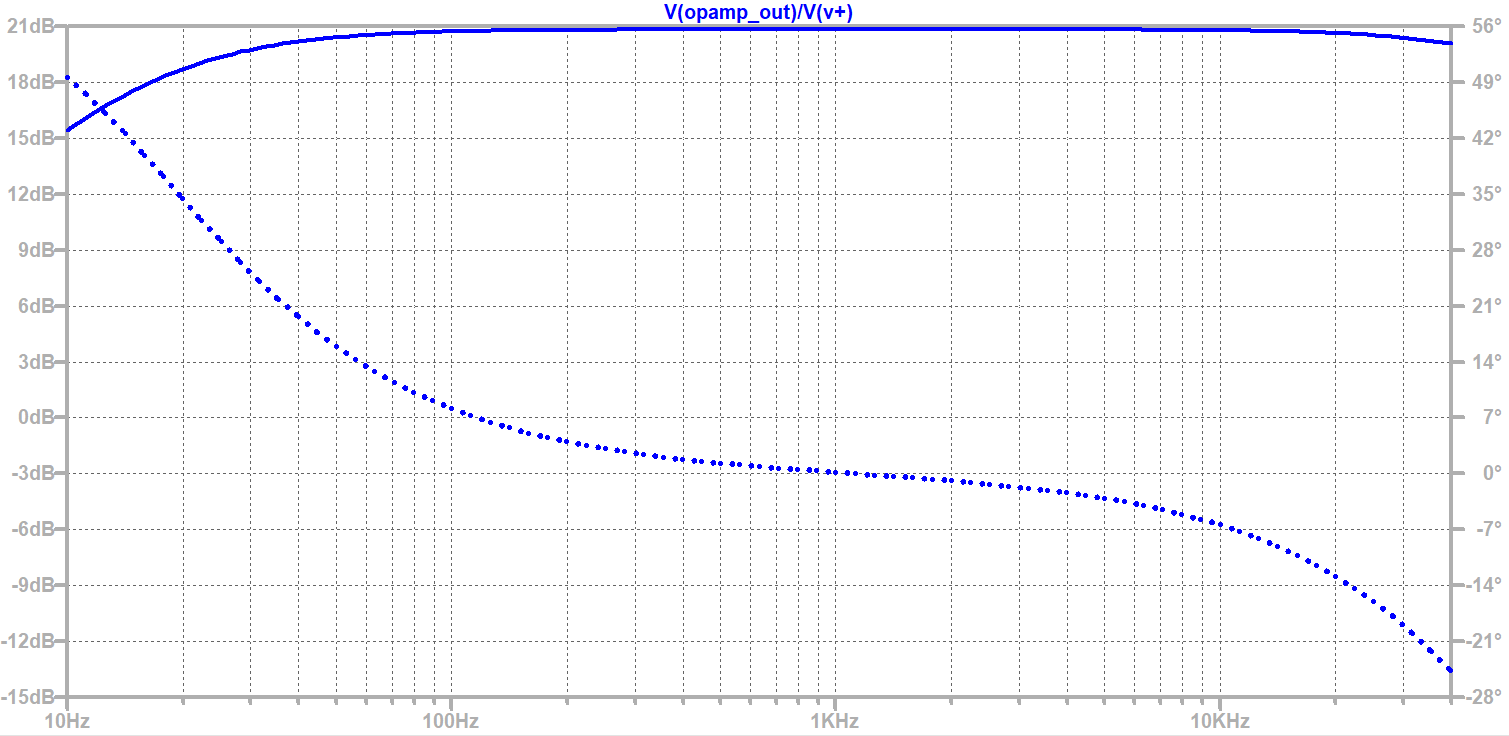
\includegraphics[scale=.4]{imagenes/bode_opamp_simulacion_300mv.png}
	\missingfigure{hacer lindo en matlab la superposicion de lo calculado, lo simulado, y lo medido}
	\caption{Transferencia del amplificador}
	\label{fig:ej5_transferencia_opamp}
\end{figure}

\subsection{Implementación del circuito y valores elegidos}
\begin{figure}[H]
	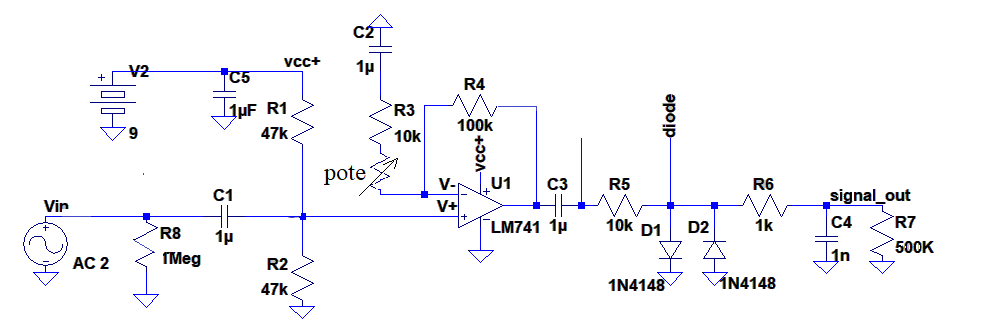
\includegraphics[scale=.4]{imagenes/circuito_final.png}
	\caption{Circuito Final con valores}
	\label{fig:ej5_circuito_final}
\end{figure}
\subsection{Simulaciones}

Se busca la respuesta en frecuencia del circuito cuando la amplificación antes de la distorsión es máxima. La amplificación o atenuación de las distintas frecuencias nos darán así una idea de que tan cuadrada la onda resultante resultará. Esto se debe a que a mayor amplificación, el corte en tensión (que es a un valor fijo determinado por los diodos) se realizara en la parte más baja de la senoidal y por ende la parte con mayor pendiente. \par
En principio, el pedal debería tener una respuesta en frecuecia característica de un filtro pasabanda, siendo las frecuencias mayormente amplificadas aquellas que se encuentran dentro del rango audible (entre 20Hz y 20kHz).\par
Debe hacerse notar, sin embargo, que el rango de frecuencias fundamentales para una guitarra eléctrica es de 80 Hz a 1.2kHz, pero que sus armónicos más importantes llegan a los 8kHz. Es por esto que la prioridad del circuito diseñado para el pedal será la de amplificar completamente hasta los 10kHz y luego ya se podrá comenzar a atenuar. La frecuencia de corte del pasa-bajos de nuestro circuito, por ende, estará cerca de este último valor.\par
Para el pasa-altos, la frecuencia de corte estará dada por los 20Hz.

\begin{figure}[H]
	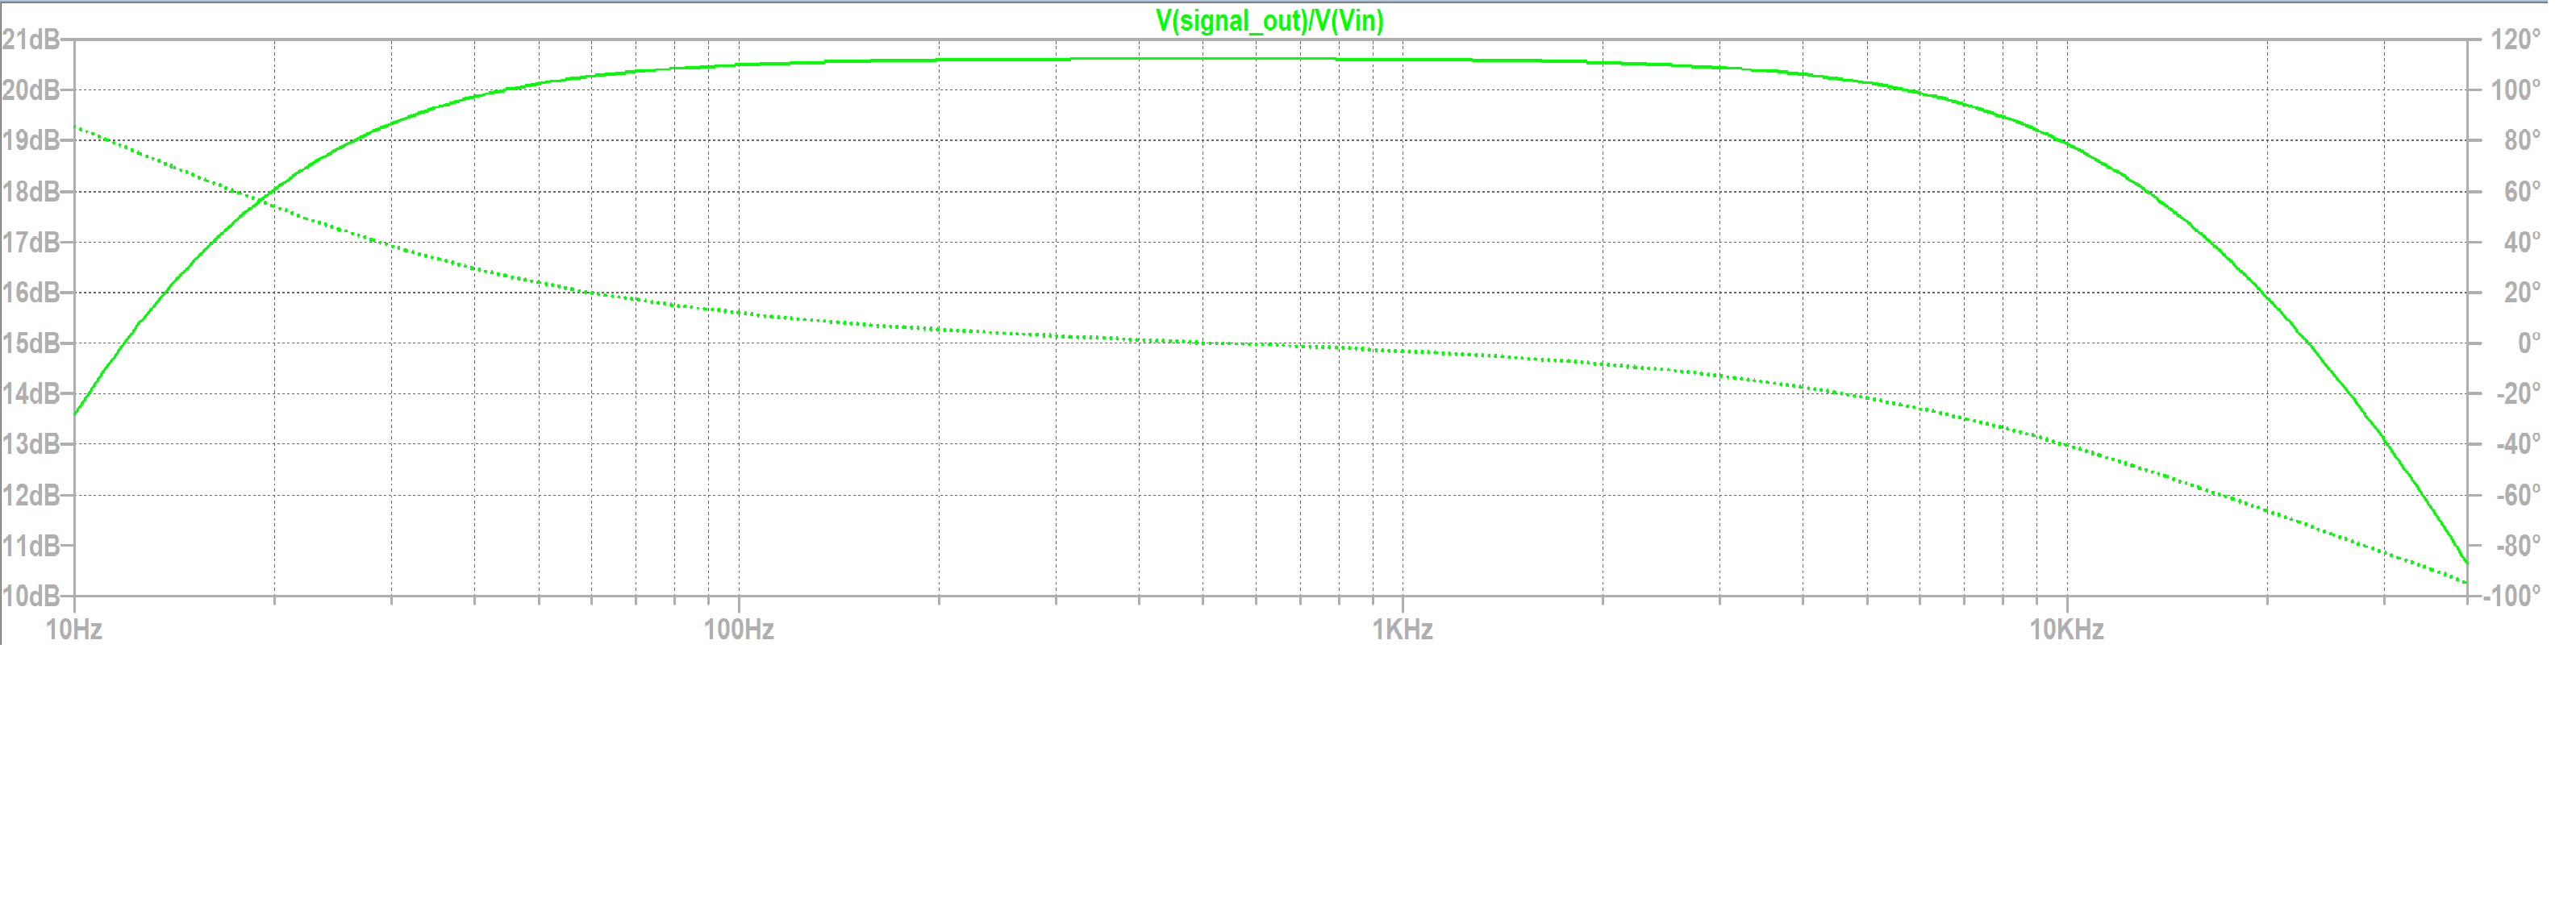
\includegraphics[scale=.4]{imagenes/Bode_simulacion.png}
	\caption{Bode simulado para la salida del circuito}
	\label{fig:ej5_Bode_simulacion}
\end{figure}
 
Se hace notar que la fase permanece aproximadamente constante en todo el rango de frecuencias de trabajo, por lo que no habrá desfasaje con la señal original para distintas frecuencias y el sonido se conservará "puro". Es decir, el sistema no distorsionará sin los diodos a las frecuencias que caen dentro del rango operativo de una guitarra.\par

Por otro lado, la salida del opamp antes de pasar por el pasabajos está dada por:
\begin{figure}[H]
	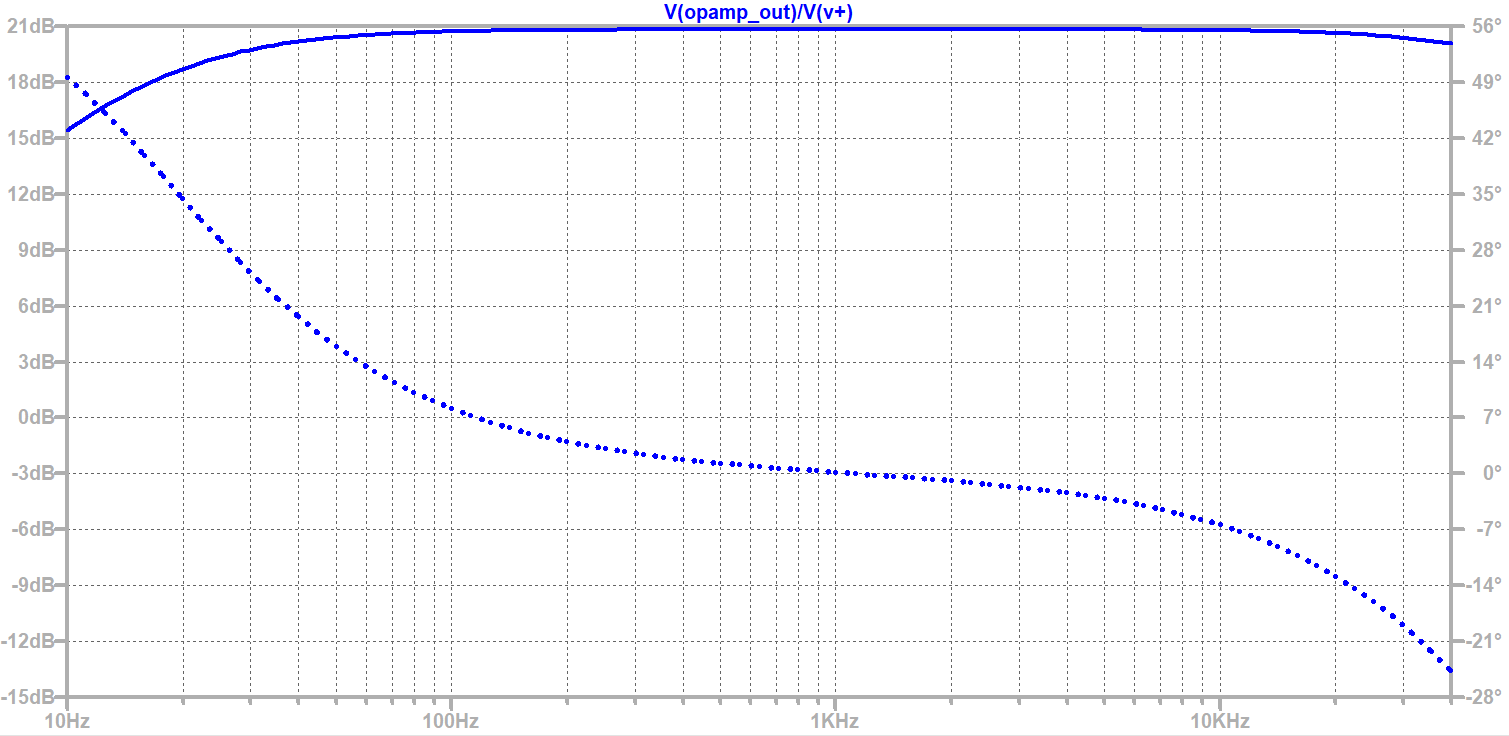
\includegraphics[scale=.4]{imagenes/bode_opamp_simulacion_300mv.png}
	\caption{Bode simulado para la salida del opamp}
	\label{fig:ej5_bode_opamp_simulacion_300mv}
\end{figure}

\subsection{Mediciones}

Los datos a partir de los cuales se construyó el siguiente bode pueden encontrarse en el anexo.

\begin{figure}[H]
	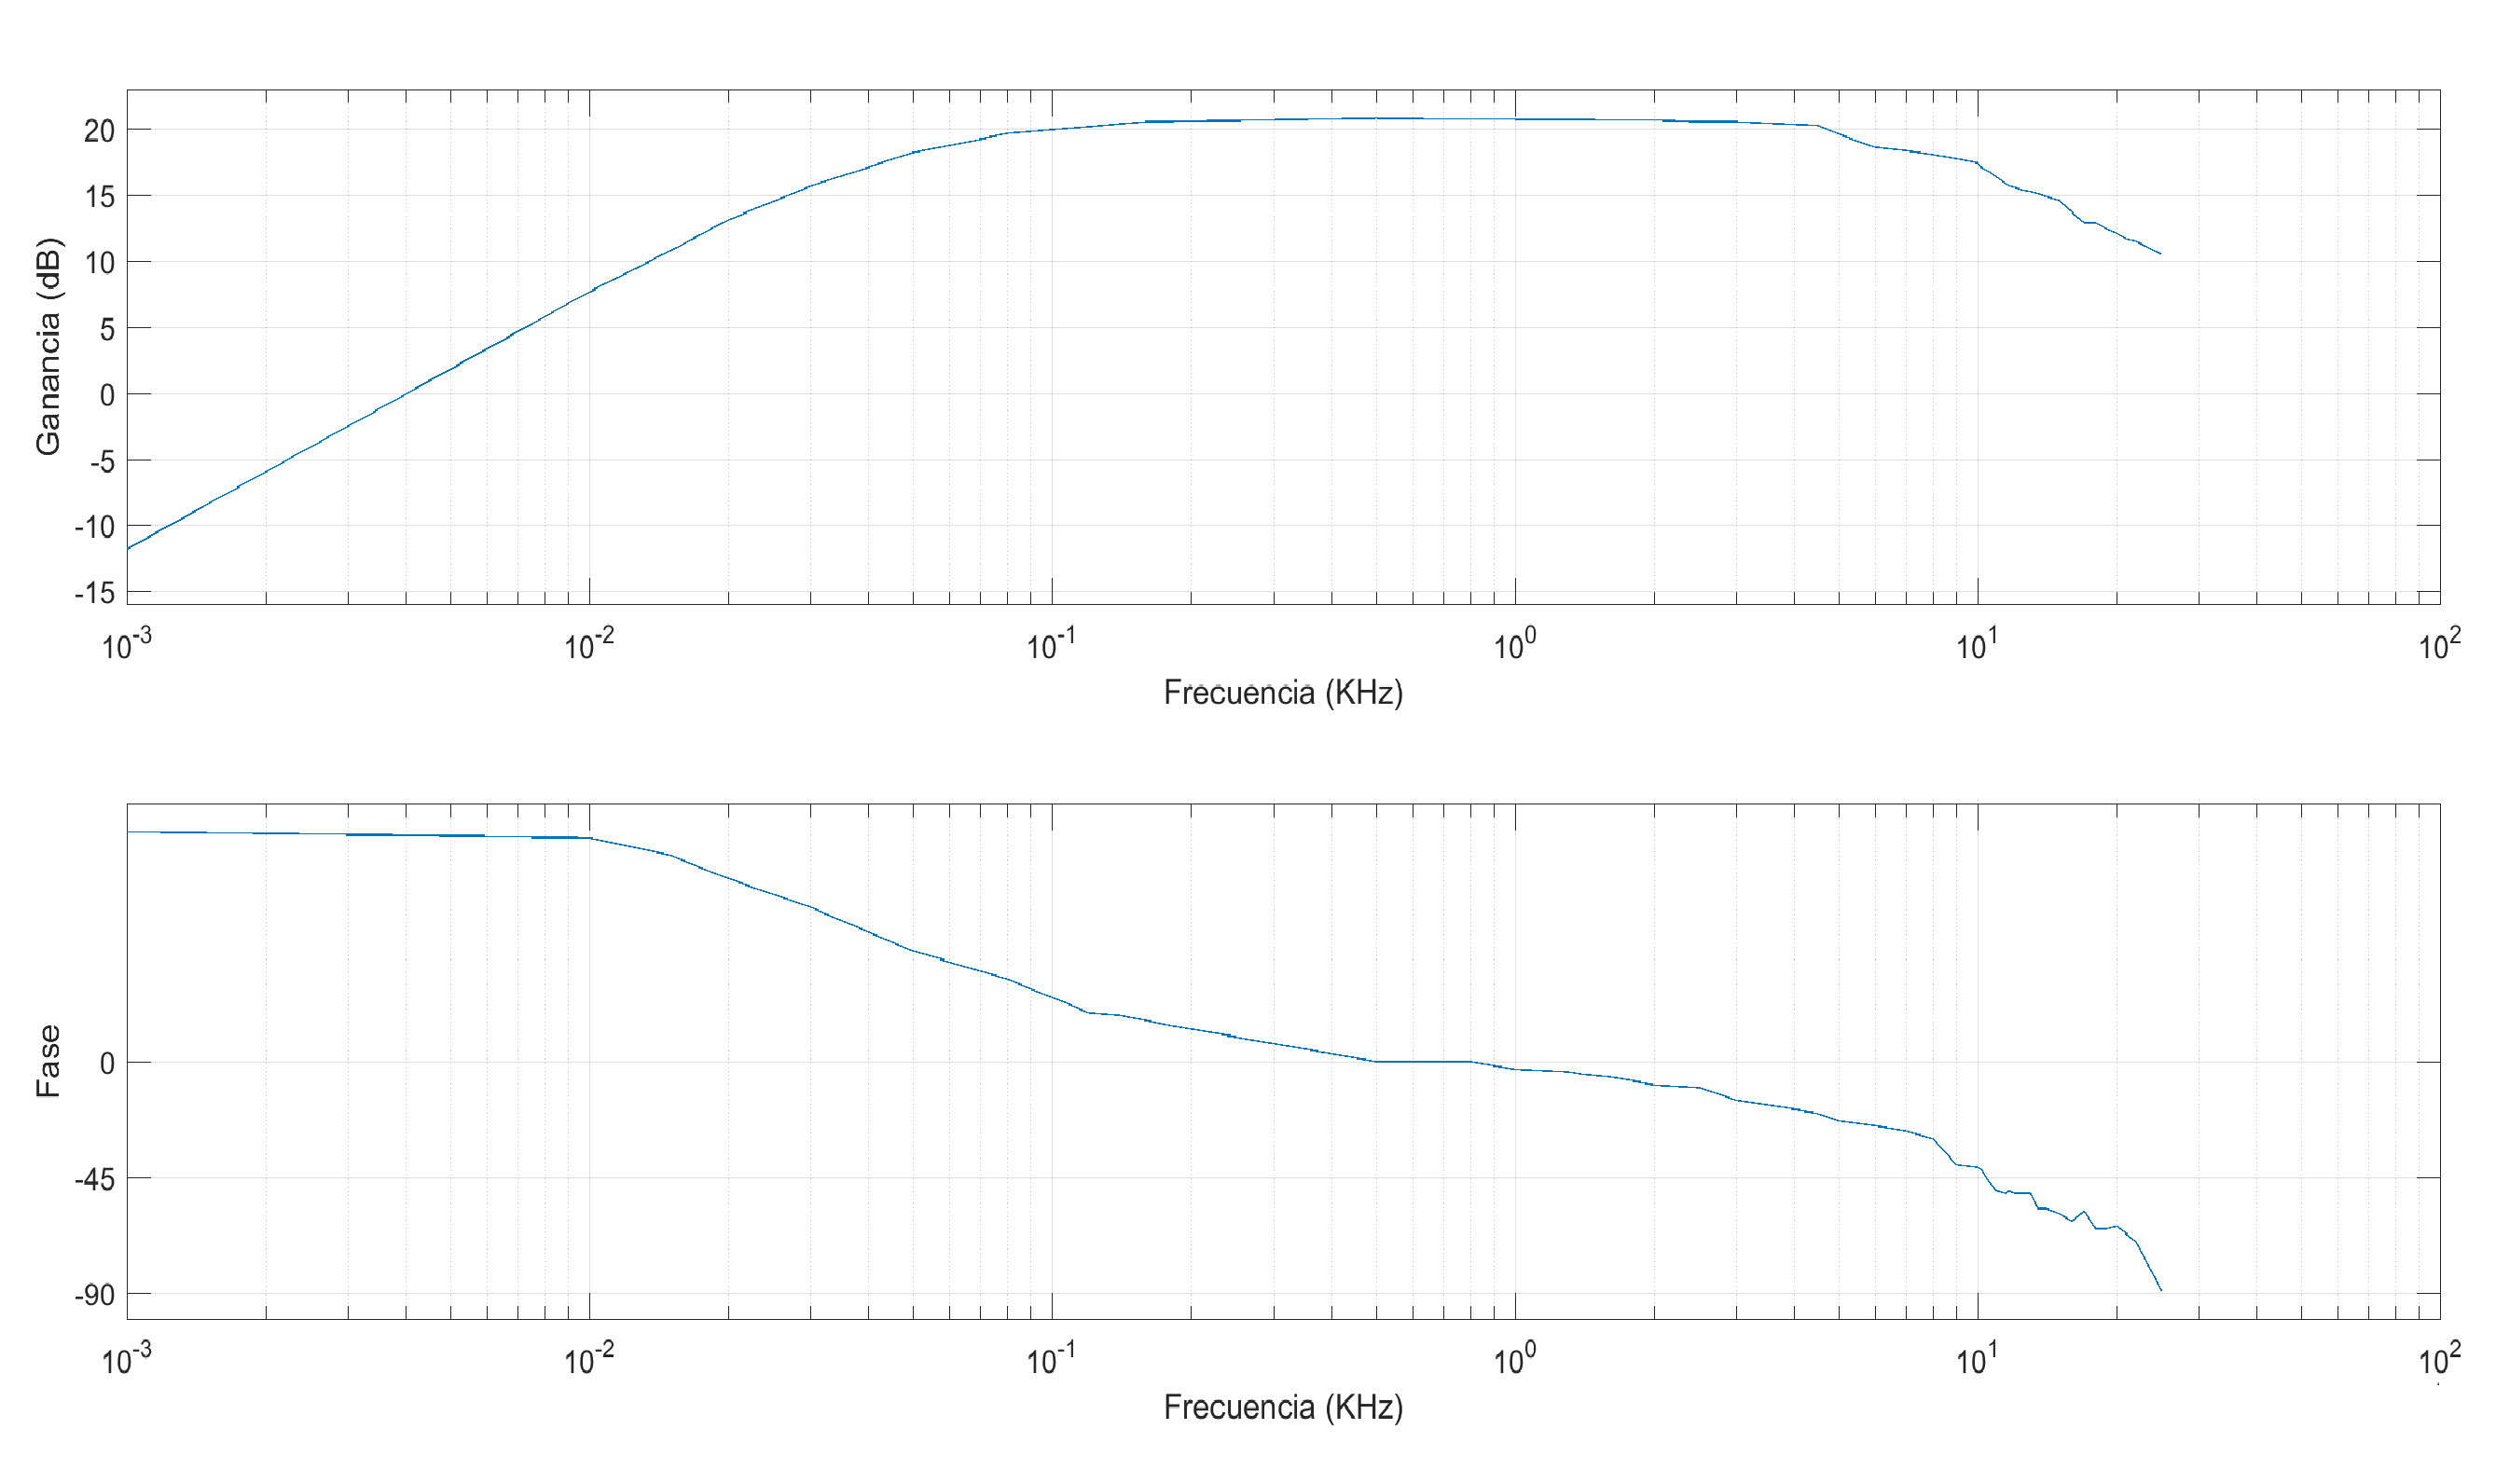
\includegraphics[scale=.4]{imagenes/bode_mediciones.png}
	\caption{Bode medido}
	\label{fig:ej5_bode_mediciones}
\end{figure}

Se aprecia una respuesta en frecuencia muy similar a la simulada, con una ganancia máxima de 21 dB y un ancho de pasabanda que se corresponde con la simulación, pudiéndose notar que la frecuencia de corte del pasa-altos resulta ser efectivamente un valor no superior a los 80 Hz y para el pasa-bajos la frecuencia de corte está claramente en 10kHz o en un valor superior a esta. \par
Sin embargo, se puede observar que el desfasaje no resulta ser la constante aproximada que se había mencionado en las simulaciones, por lo que hay una distorsión en fase no deseada. 

\end{document}
